\Tsubsection{UI3 Proceso concluido} 
%------------------------------------Objetivo----------------------------------%
\begin{large}
  \textbf{Objetivo}\\
\end{large}


Informal al usuario que la recolección y clasificación ha concluido y brinda un punto de acceso para visualizar los resultados de la consulta.\\

%------------------------------------Descripción---------------------------------%
\begin{large}
  \textbf{Descripción}\\
\end{large}

La Pantalla \ref{fig:UI3} muestra un mensaje flotante con la siguiente redacción: \textbf{Noticias listas para ser mostradas}, el cual informa al usuario que el proceso de recolección y clasificación ha concluido, \textit{i.e} ya se pueden mostrar las noticias clasificadas de la sección elegida. En la parte inferior se muestra el botón \textbf{Cancelar} y \textbf{Continuar}.  \\

%-----------------------------------Salidas------------------------------------%
\begin{large}
  \textbf{Salidas}
\end{large}

\begin{itemize}

  \item Ninguno

\end{itemize}

%------------------------------------Comandos----------------------------------%

\textbf{Comandos}

\begin{enumerate}

  \item \textbf{Cancelar}: Detiene el proceso de recolección y clasificación, re-direcciona a la pantalla \Tref{UI1}{UI1 Inicio}.
  \item \textbf{Continuar}: Permite avanzar para visualizar las noticias clasificadas de la sección elegida en la pantalla \Tref{UI4}{UI4 Resultados de consulta}

\end{enumerate}

%------------------------------------Referencia----------------------------------%
\begin{large}
  \textbf{Referenciado por}
\end{large}

\begin{itemize}

  \item \Tref{CU1}{CU1 Recolectar noticias}
  \item \Tref{CU4}{CU4 Mostrar resultados}

\end{itemize}  

%----------------------------------------Pantalla--------------------------------%

\begin{figure}\Tlabel{UI3}
  \centering
	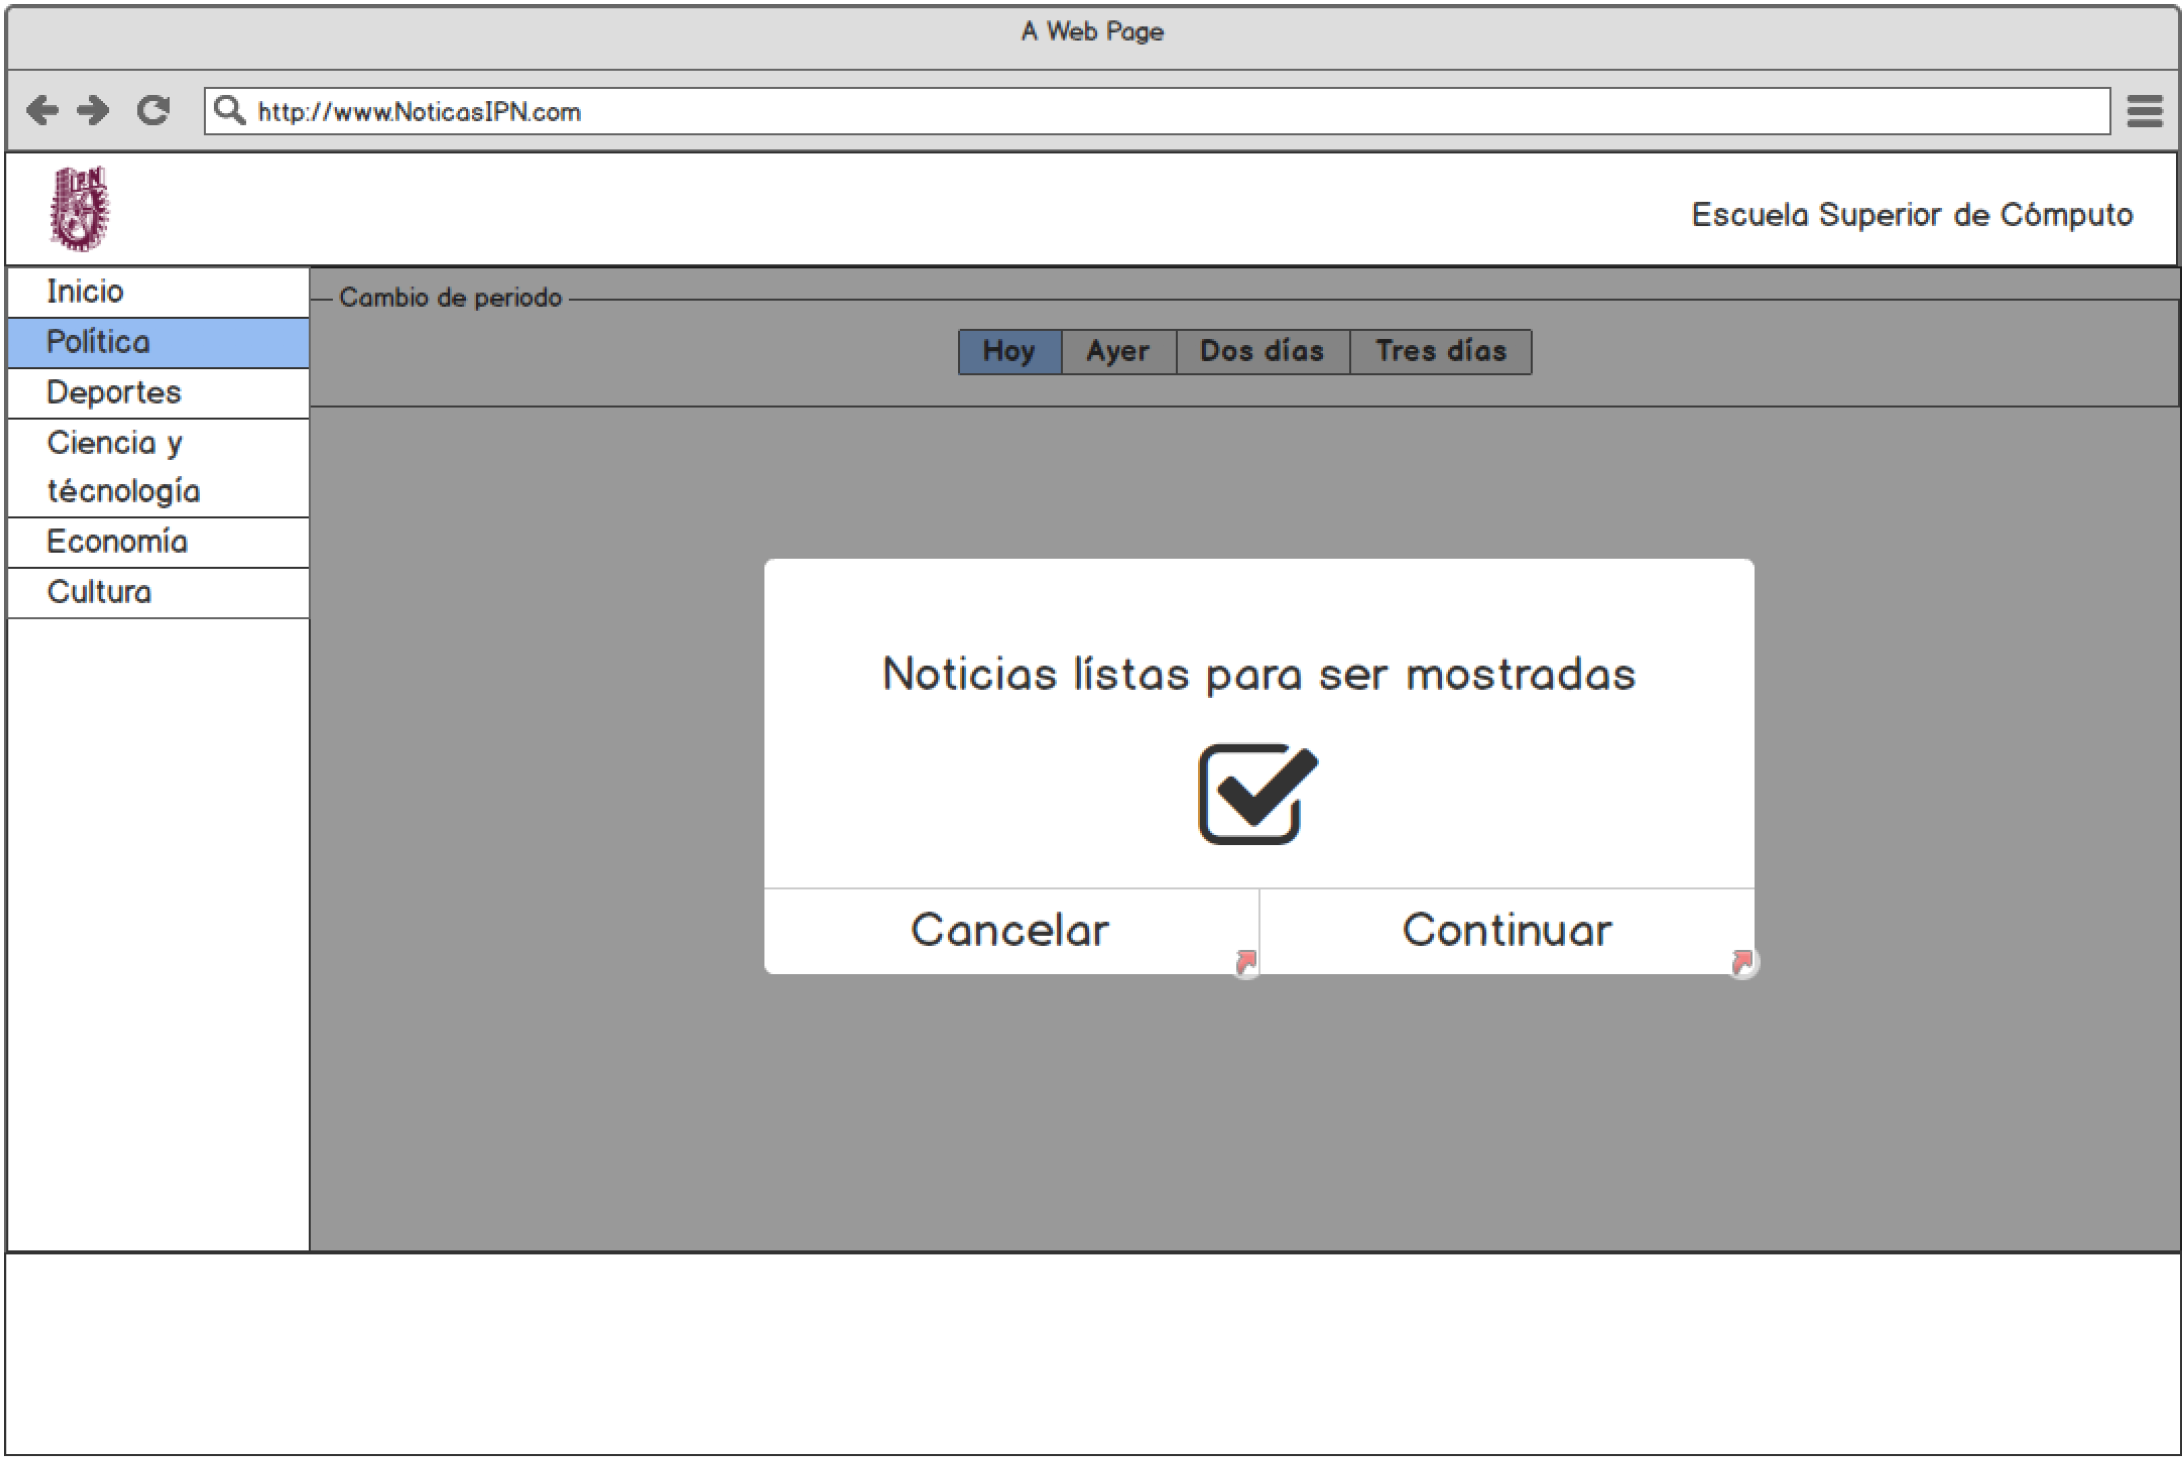
\includegraphics[scale=.35]{imagenes/Pantallas/UI3}
  \caption{Pantalla UI3 Proceso concluido}
  \label{fig:UI3}
\end{figure}
